\documentclass[xcolor=x11names,12pt]{beamer}
%\usetheme[secheader]{Boadilla} 
\mode<presentation>{\usetheme{I6pd2}}

\usepackage{multicol} 
\usepackage[utf8]{inputenc}
\usepackage[english]{babel}
\usepackage{grffile}
\usepackage{listings}
\usepackage{multirow}
\usepackage{amsmath}
\usepackage{pifont}
\usepackage{slashbox}
\usepackage{marvosym}
\usepackage[ruled]{algorithm2e}
\usepackage{pgf}
\usepackage{pgfcore}
\usepackage{pgfbaseimage}
\usepackage{pgfbaselayers}
\usepackage{pgfbasepatterns}
\usepackage{pgfbaseplot}
\usepackage{pgfbaseshapes}
\usepackage{pgfbasesnakes}
\usepackage{tikz} 

\tikzset{normal/.style={ 
% The shape: 
rectangle,minimum size=6mm,rounded corners=3mm, 
% The rest 
very thick,draw=black!50, 
top color=white,bottom color=black!20, 
font=\ttfamily}}
\tikzset{arduino/.style={ 
% The shape: 
rectangle, 
% The size: 
minimum size=6mm, 
% The border: 
very thick, 
draw=blue!50!black!50, % 50% red and 50% black, 
% and that mixed with 50% white 
% The filling: 
top color=white, % a shading that is white at the top... 
bottom color=blue!50!black!20, % and something else at the bottom 
% Font 
font=\itshape 
}}
\tikzset{enceinte/.style={ 
% The shape: 
rectangle, 
% The size: 
minimum size=6mm, 
% The border: 
very thick, 
draw=yellow!90!black!50, % 50% red and 50% black, 
% and that mixed with 50% white 
% The filling: 
top color=white, % a shading that is white at the top... 
bottom color=yellow!90!black!20, % and something else at the bottom 
% Font 
font=\itshape 
}}

\tikzset{ordi/.style={ 
% The shape: 
rectangle, 
% The size: 
minimum size=6mm, 
% The border: 
very thick, 
draw=green!90!black!50, % 50% red and 50% black, 
% and that mixed with 50% white 
% The filling: 
top color=white, % a shading that is white at the top... 
bottom color=green!90!black!20, % and something else at the bottom 
% Font 
font=\itshape 
}}

\usetikzlibrary{through,shapes,arrows,decorations.pathmorphing,backgrounds,positioning,fit} 

\newcommand{\argmin}{\mathop{\mathrm{min}}}
\usepackage[orientation=portrait,size=a0,scale=1.4]{beamerposter}


\newcommand{\conf}[1]{\newcommand{\insertconf}{#1}}
\newenvironment{WholeWidthBox}[1]{
  \begin{columns}
    \begin{column}{0.98\textwidth}
      \begin{block}{#1}
        \begin{hfill}
}{
        \end{hfill}
      \end{block}
    \end{column}
  \end{columns}
}

\newcommand{\TwoBoxes}[7]{%Width1 Title1 Content1 Width2 Title2 Content2 MinHeight
  \begin{columns}
    \begin{column}{#1\textwidth}
      \begin{block}{#2}
        \begin{columns}
          \begin{column}{0.001\textwidth}
            \vspace{#7}
          \end{column}
          \begin{column}{\textwidth}
            \centering
            #3
          \end{column}
        \end{columns}       
      \end{block}
    \end{column}
    
    \begin{column}{#4\textwidth}
      \begin{block}{#5}
        \begin{columns}
          \begin{column}{0.001\textwidth}
            \vspace{#7}
          \end{column}
          \begin{column}{\textwidth}
            \centering
            #6
          \end{column}
        \end{columns}       
      \end{block}
    \end{column}
  \end{columns}
}


%Start of document



\tikzstyle{state}=[circle,
thick,
minimum size=1.0cm,
draw=blue!80,
fill=blue!20]
\tikzstyle{action}=[rectangle,thick,
minimum size=1.0cm,
draw=orange!80,
fill=orange!20]
\tikzstyle{element}=[rectangle,
line width=1.5mm,
minimum size=1.0cm,
draw=blue!80,
fill=blue!20]
\tikzstyle{action}=[rectangle,
line width=1.5mm,
minimum size=1.0cm,
draw=orange!80,
fill=orange!20]



\conf{NIPS 2012}
\title{Inverse Reinforcement Learning through Structured Classification}
\author{\underline{Edouard Klein}$^{\dag\ddag}$, Matthieu Geist$^\dag$, Bilal Piot$^{\dag\textrm{\Ankh}}$ and Olivier Pietquin$^{\dag\textrm{\Ankh}}$\\\texttt{firstname.lastname@supelec.fr}}
\date{\today}
\institute[Supélec]{$\dag$Equipe IMS/MaLIS (Supélec), France\\$\ddag$Equipe ABC UMR 7503 (Loria-CNRS), France\\\Ankh UMI 2958 (GeorgiaTech-CNRS)}
\newlength{\columnheight}
\setlength{\columnheight}{105cm}


\begin{document}
\begin{frame}

%%%%%%%%%%%%% DEBUT PREMIERE LIGNE %%%%%%%%%%%%%%%%%
\begin{WholeWidthBox}{1. Introduction}
  The inverse reinforcement learning (IRL) problem can be defined as inferring a reward for which a demonstrated expert behavior is optimal. We introduce a new algorithm, SCIRL, whose principle is to use the so-called feature expectation of the expert as the parameterization of the score function of a multi-class classifier. This approach produces a reward function for which the expert policy is provably near-optimal. Contrary to most of existing IRL algorithms, SCIRL does not require solving a single time the direct RL problem. Moreover, up to the use of some heuristic, it may work with only trajectories sampled according to the expert behavior. This is illustrated on toy problems.
\end{WholeWidthBox}

\vfill
%%%%%%%%%%%% DEBUT DEUXIEME LIGNE %%%%%%%%%%%%%%%%%%

\TwoBoxes{.48}{2. Setting}{
  \begin{columns}
    \begin{column}{.48\textwidth}
      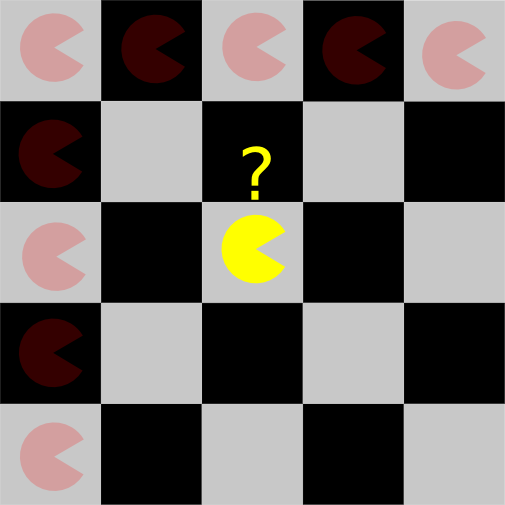
\includegraphics{Agent003.png}
    \end{column}
    \begin{column}{.48\textwidth}
      \begin{itemize}
      \item Expert's trace
      \item $MDP\backslash R $
      \item $\pi^*(s) \in \arg\max_{a\in A}Q^*(s,a)$
      \item $R(s) = \theta^T\psi(s)$
      \end{itemize}
      
    \end{column}
  \end{columns}
}
{.48}{3. Assumptions and Goal}{
  \begin{itemize}
  \item Assumptions
    \begin{itemize}
    \item The expert is a RL agent
    \item One can access the expert's trace
    \item The agent has the same abilities as the expert
    \end{itemize}
  \item Goal : Infer the expert's reward
    \begin{itemize}
    \item apprenticeship of the expert's task
    \item Generalization of the policy over never-seen-before states
    \item Useful when rewards are hard to tune ({\it e.g.}, driving)
    \end{itemize}
  \end{itemize}
}
{15cm}
\vfill
%%%%%%%%%%%%%%%%%%%%%%%%%%%%%%%% TROISIEME, quatrième, cinquième et sixième LIGNES
\begin{columns}
  \begin{column}{.48\textwidth}
    \begin{block}{4. Expert}
      \begin{columns}
        \begin{column}{0.001\textwidth}
          \vspace{8cm}
        \end{column}
        \begin{column}{\textwidth}
          \begin{itemize}
          \item The expert is optimal : $\pi_E(s) = \arg\max\limits_{a} Q^{\pi_E}(s,a)$
          \item w.r.t. a linearly parametrized reward : $Q^\pi(s_t,a) = \theta^T\mu^\pi(s_t,a)$
          \item thus : \tikz{\node[fill=red!30,draw=red,ultra thick,rounded corners]{$\pi_E(s) \in \arg\max\limits_{a} \theta^T\mu^{\pi_E}(s,a)$};}
          \end{itemize}
        \end{column}
      \end{columns}
    \end{block}
    \vspace{1cm}
    \begin{block}{6. Linearly parametrized score function based classifiers}
      \begin{columns}
        \begin{column}{0.001\textwidth}
          \vspace{8cm}
        \end{column}
        \begin{column}{\textwidth}
          \begin{itemize}
          \item A score function : $g_s(x) \in \arg\max\limits_{y\in\mathcal{Y}}s(x,y)$
          \item which is linearly parametrized : $s(x,y) = \theta^T \phi(x,y)$
          \item gives : \tikz{\node[fill=red!30,draw=red,ultra thick,rounded corners]{$g_s(x) \in \arg\max\limits_{y\in\mathcal{Y}}\theta^T\phi(x,y)$};}
          \end{itemize}
        \end{column}
      \end{columns}             
    \end{block}
    \vspace{1cm}
    %% \begin{block}{Putting it all together}
    %%   \begin{equation*}
    %%     \mathcal{X} \equiv S, \mathcal{Y} \equiv A, s\equiv Q^{\pi_E} \Rightarrow \phi \equiv \mu^{\pi_E}
    %%   \end{equation*}
    %% \end{block}
    \vfill
    \begin{block}{7. Pseudo-code}
      \resizebox{.95\columnwidth}{!}{
        \begin{algorithm}[H]%[tbh]
          %\small
          %\SetVline
          \caption{SCIRL algorithm}
          \label{algo:scirl}
          %
          \BlankLine
          \emph{\textbf{Given}} a training set $\mathcal{D} = \{(s_i,a_i=\pi_E(s_i))_{1\leq i\leq N}\}$,
          an estimate $\hat{\mu}^{\pi_E}$ of the expert feature expectation $\mu^{\pi_E}$ and a classification algorithm\;
          %
          \BlankLine
          \emph{\textbf{Compute}} the parameter vector $\theta_c$ using the
          classification algorithm
          fed with the training set $\mathcal{D}$ and considering the parameterized score function
          $\theta^T\hat{{ \mu}}^{\pi_E}(s,a)$\;
          %
          \BlankLine
          \emph{\textbf{Output}} the reward function $R_{\theta_c}(s) = \theta_c^T\psi(s)$ \;
        \end{algorithm}
      }
    \end{block}
  \end{column}
  \begin{column}{.48\textwidth}
    \begin{block}{5. Feature Expectation}
        \begin{equation*}
          Q^\pi(s_t,a) = E\left[\left.\sum\limits_{i}\gamma^i r_{t+i}\right|\pi,s_t,a\right] = \theta^T\underbrace{E\left[\left.\sum\limits_{i}\gamma^i \psi(s_{t+i})\right|\pi,s_t,a\right]}_{\color{red}\mu^\pi(s_t,a)}
        \end{equation*}
    \end{block}
    \vfill
    \begin{block}{8. Error bound}
      With concentration coefficient $C_f$, classification error $\epsilon_C$ and $\bar{\epsilon}_Q$ a measure of the quality of our estimate of $\mu^{\pi_E}$ :
      \begin{equation*}
        0\leq
        \mathop{E}_{s\sim\rho_E}[V^*_{R_{\theta_c}}(s)-V^{\pi_E}_{R_{\theta_c}}(s)]
        \leq \frac{C_f}{1-\gamma}\left(\bar{\epsilon}_Q +
        \epsilon_c\frac{2\gamma\|R_{\theta_c}\|_\infty}{1-\gamma}
        \right)
      \end{equation*}
    \end{block}
    \vfill
    \begin{block}{9. Highway}
      \begin{columns}
        \begin{column}{0.001\textwidth}
          \vspace{7cm}
        \end{column}
        \begin{column}{\textwidth}
          \centering
          \fontsize{11pt}{11pt}\selectfont
          \resizebox{.95\columnwidth}{!}{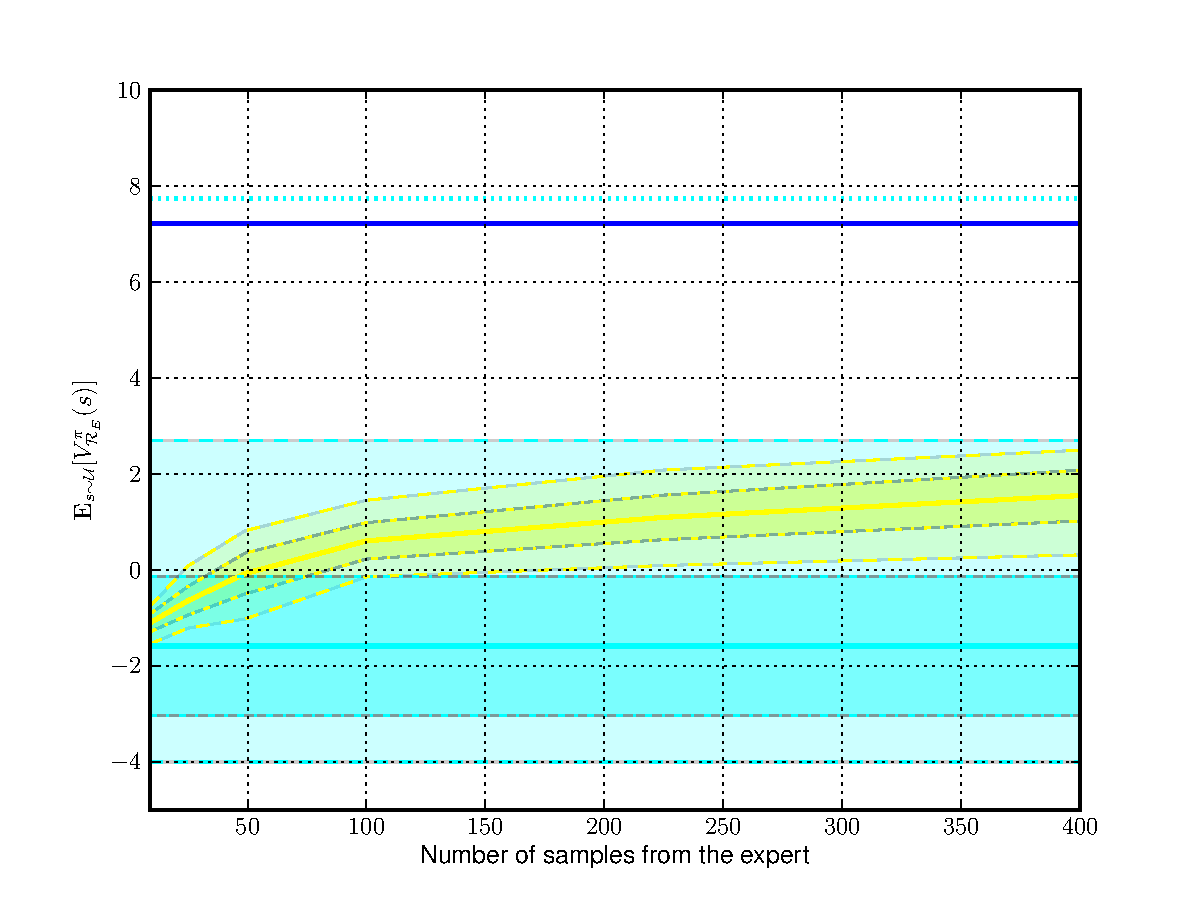
\includegraphics[width=0.47\textwidth]{Cascading_Exp5_fig2}
            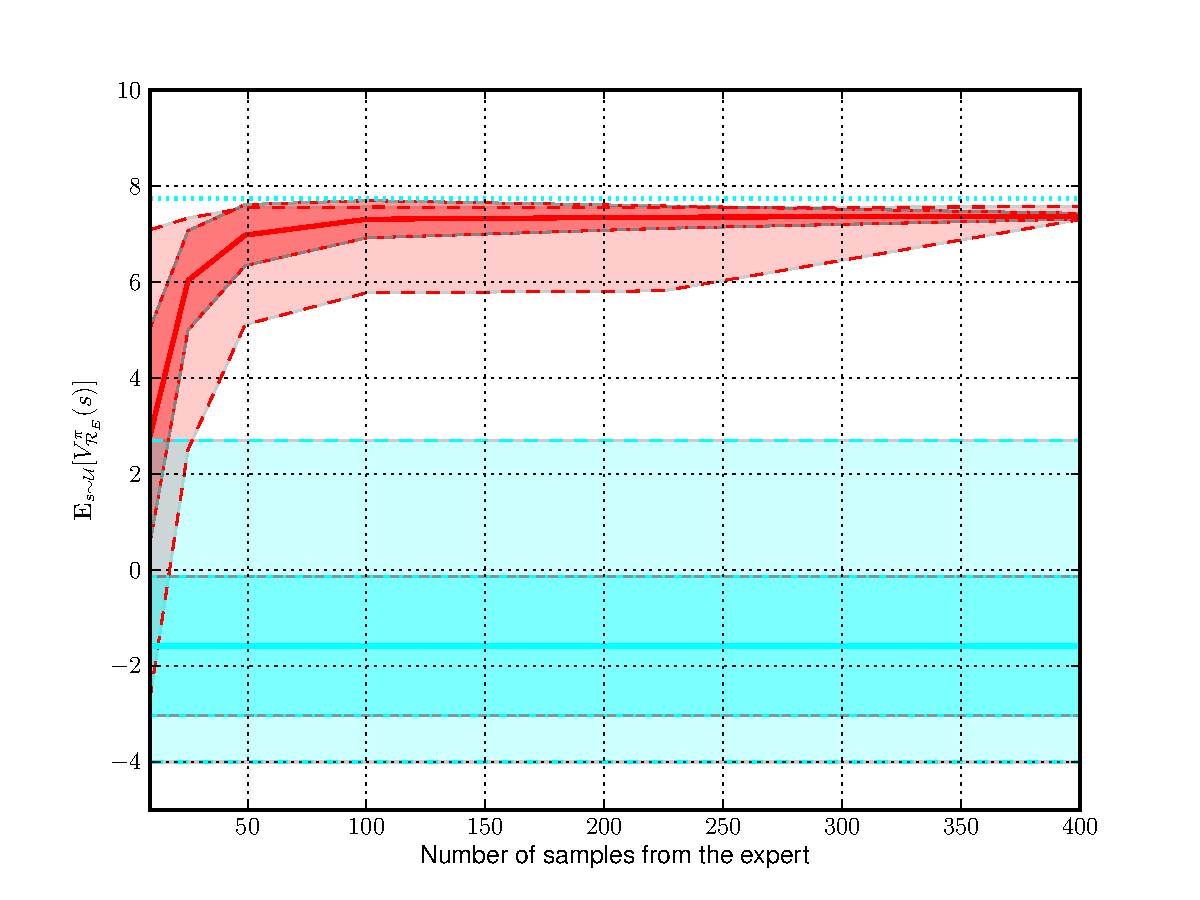
\includegraphics[width=0.47\textwidth]{SCIRL_Exp3_fig1}}
        \end{column}
      \end{columns}             
    \end{block}
  \end{column}
\end{columns}
\vfill
%%%%%%%%%%%%% Septième ligne
  \begin{columns}
    \begin{column}{.48\textwidth}
      \begin{block}{10. GridWorld}
        \centering
%        \fontsize{11pt}{11pt}\selectfont
%        \resizebox{.95\columnwidth}{!}{
%         Bli\\
\vspace{-70pt}
          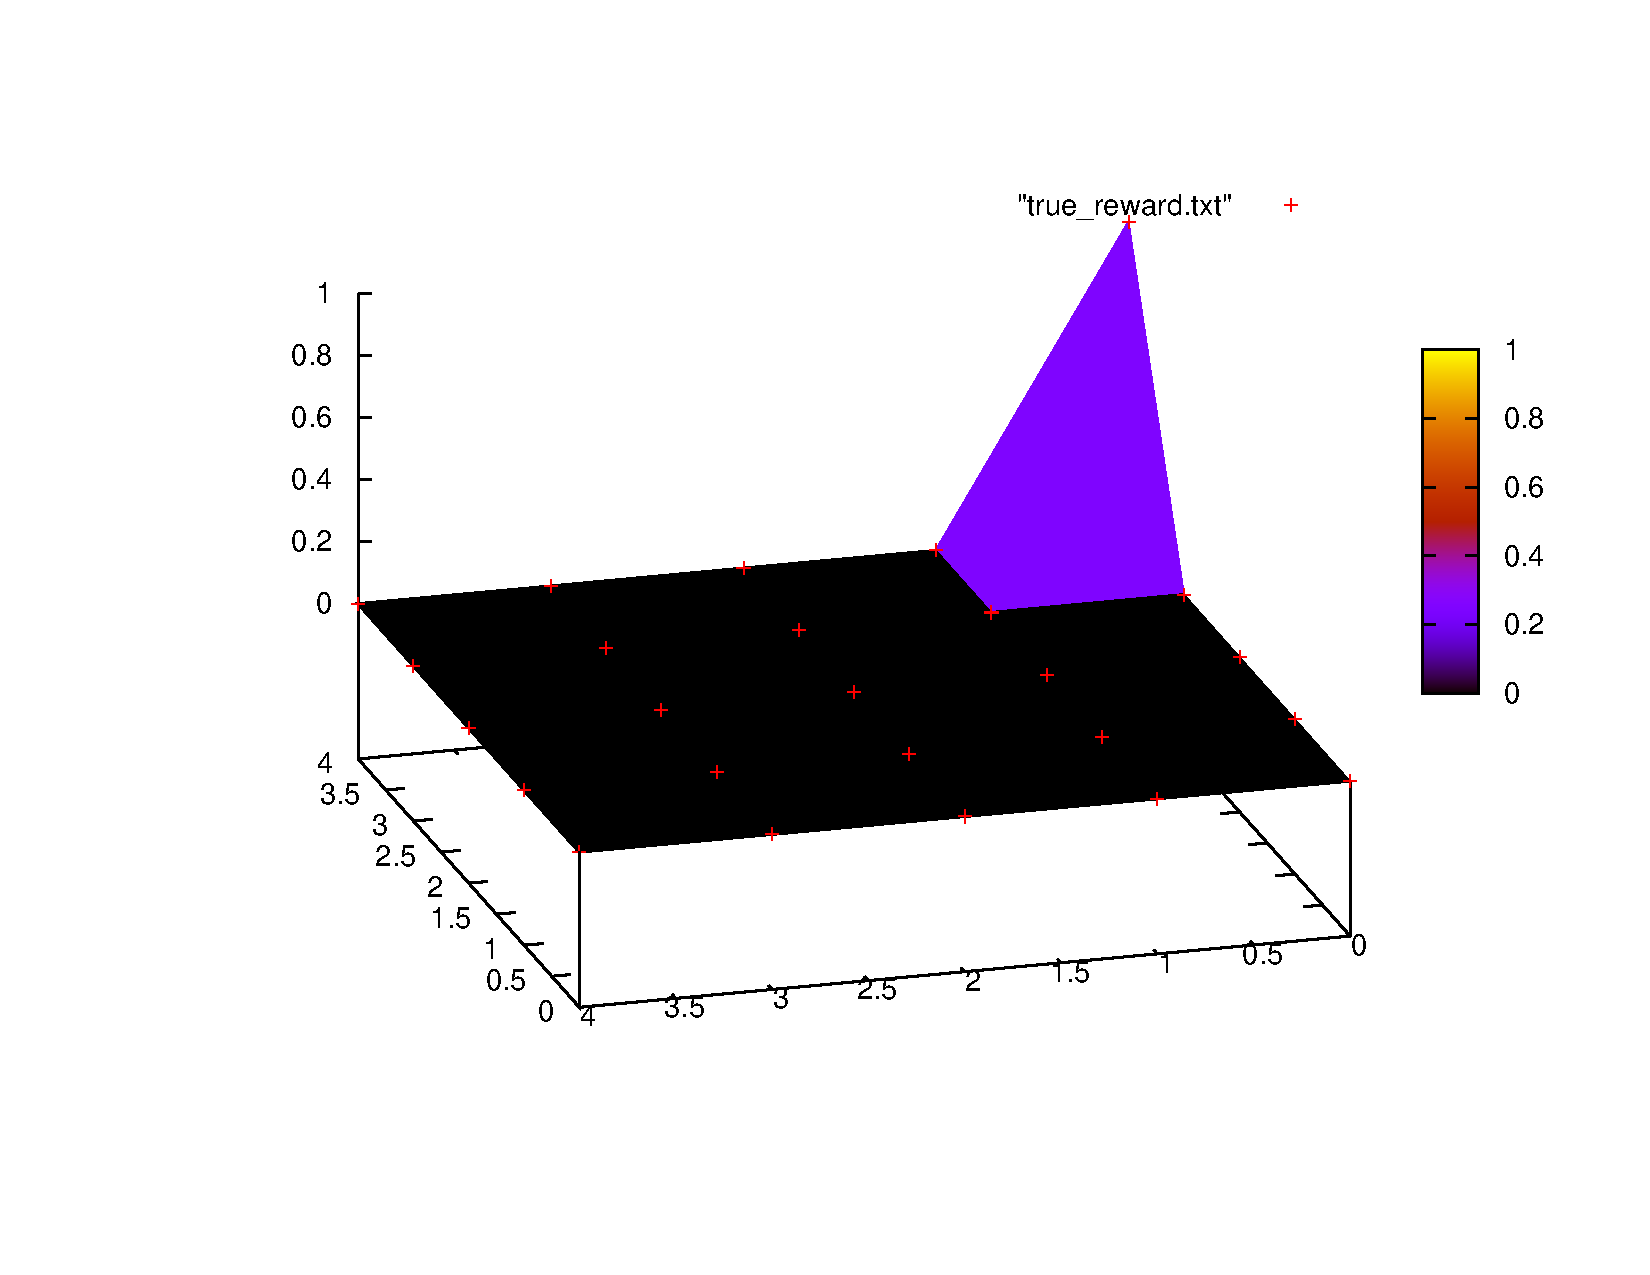
\includegraphics[width=.52\textwidth]{true_reward.pdf}\hspace{-100pt}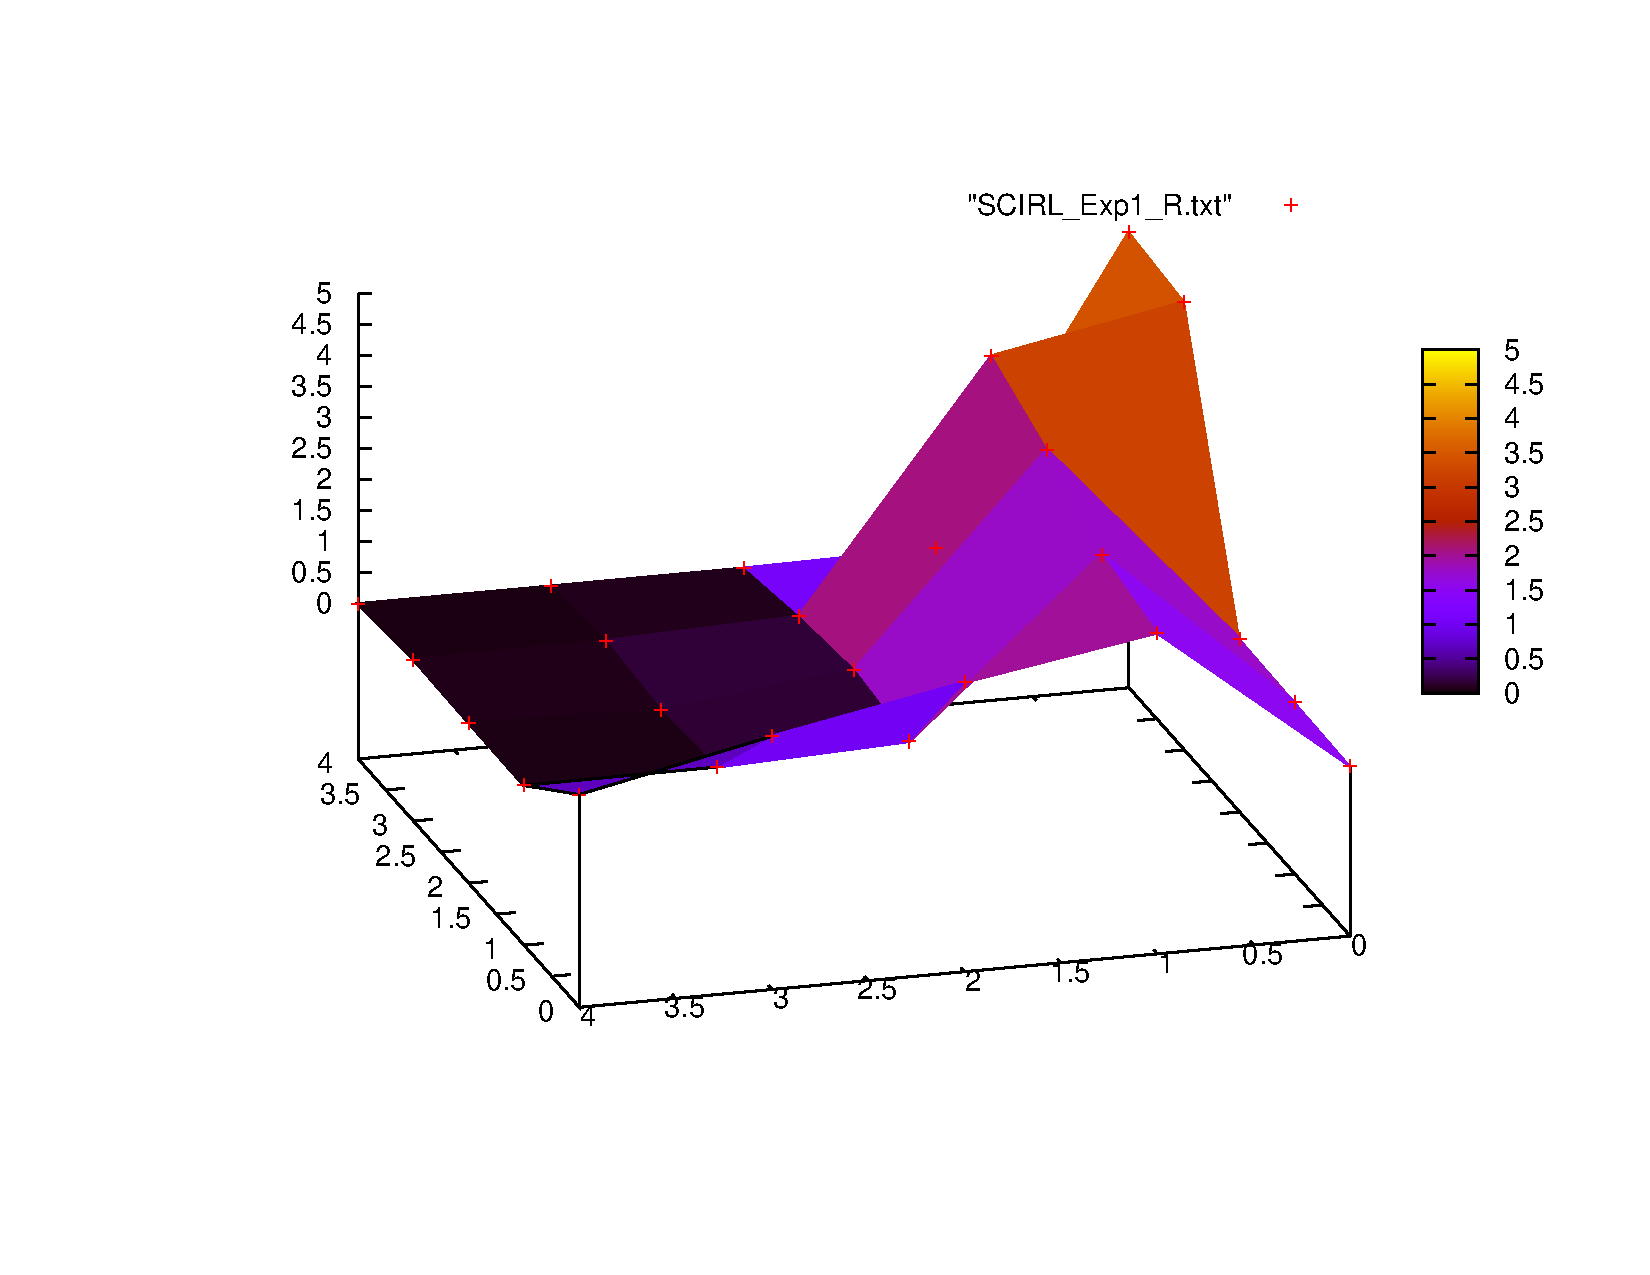
\includegraphics[width=.52\textwidth]{SCIRL_Exp1_R.pdf}\\
%          Blah
\vspace{-110pt}
          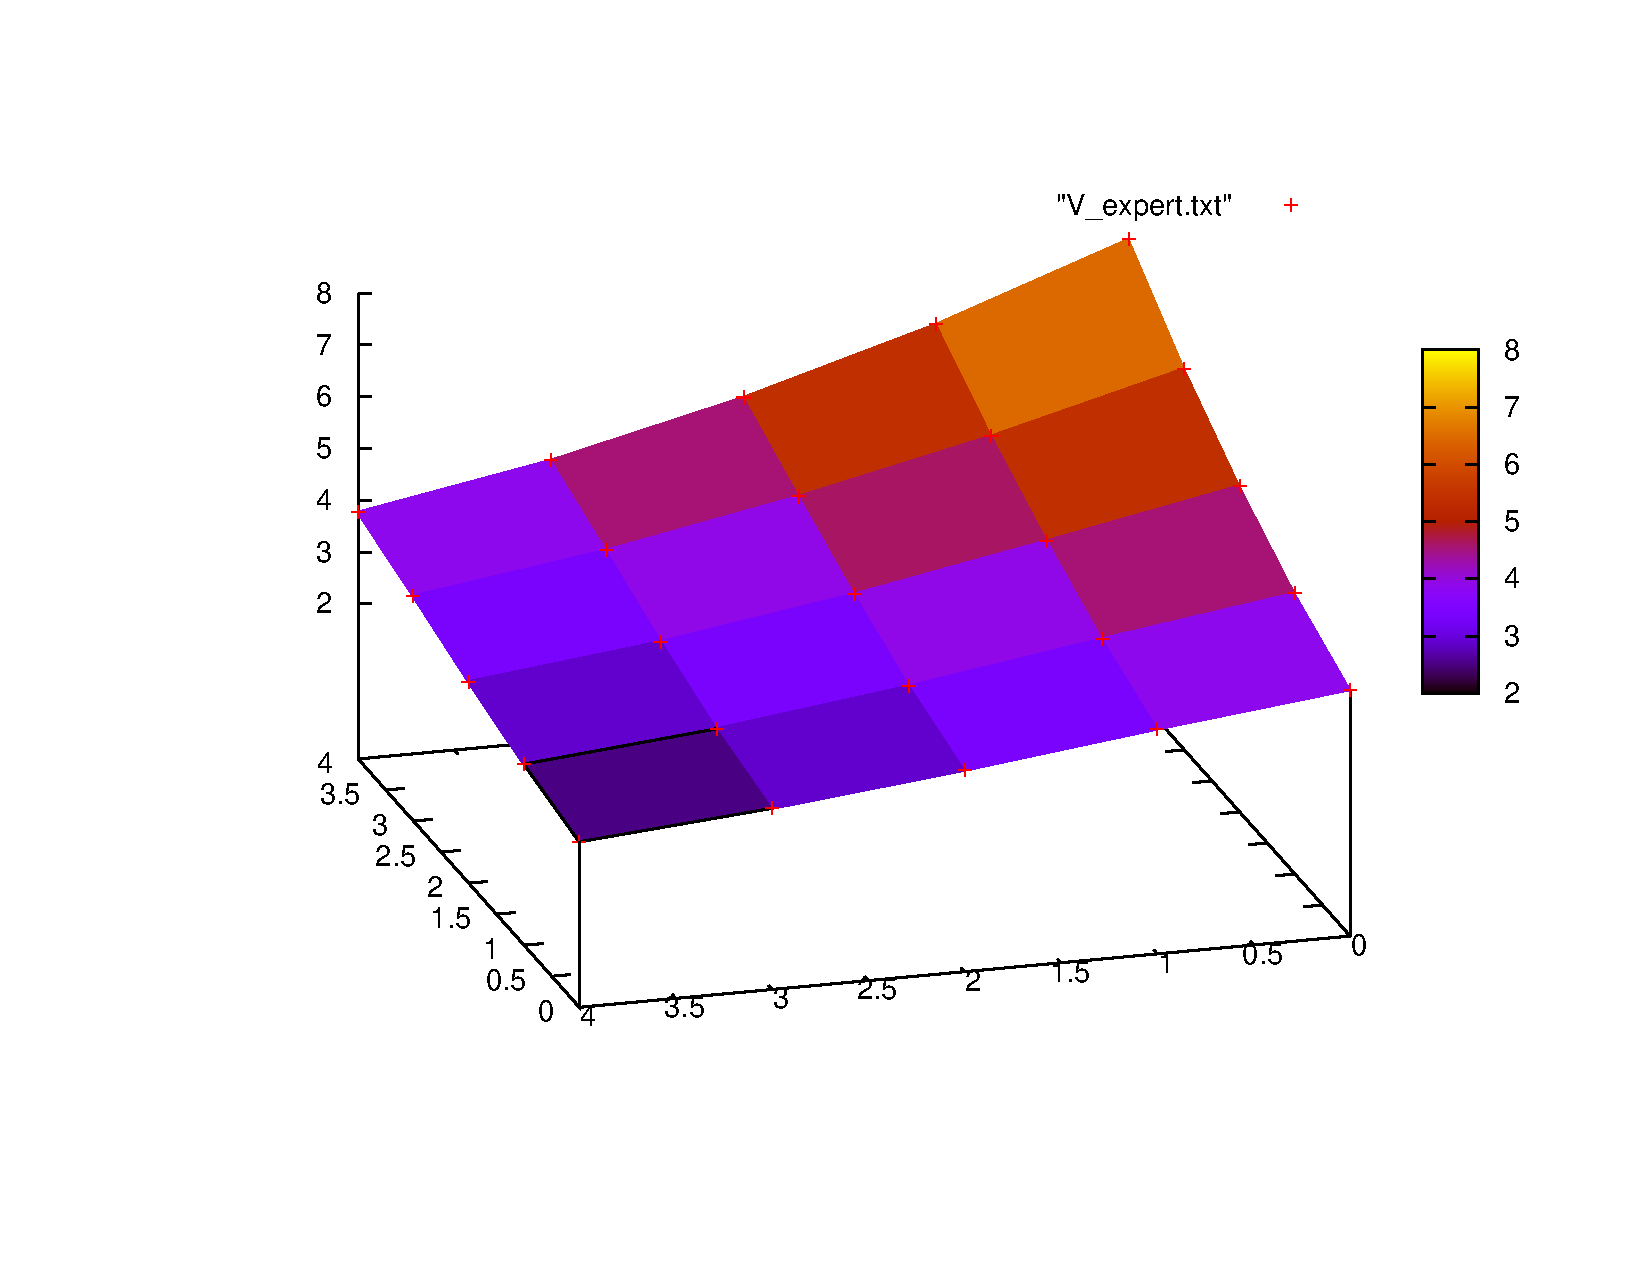
\includegraphics[width=.52\textwidth]{V_expert.pdf}\hspace{-100pt}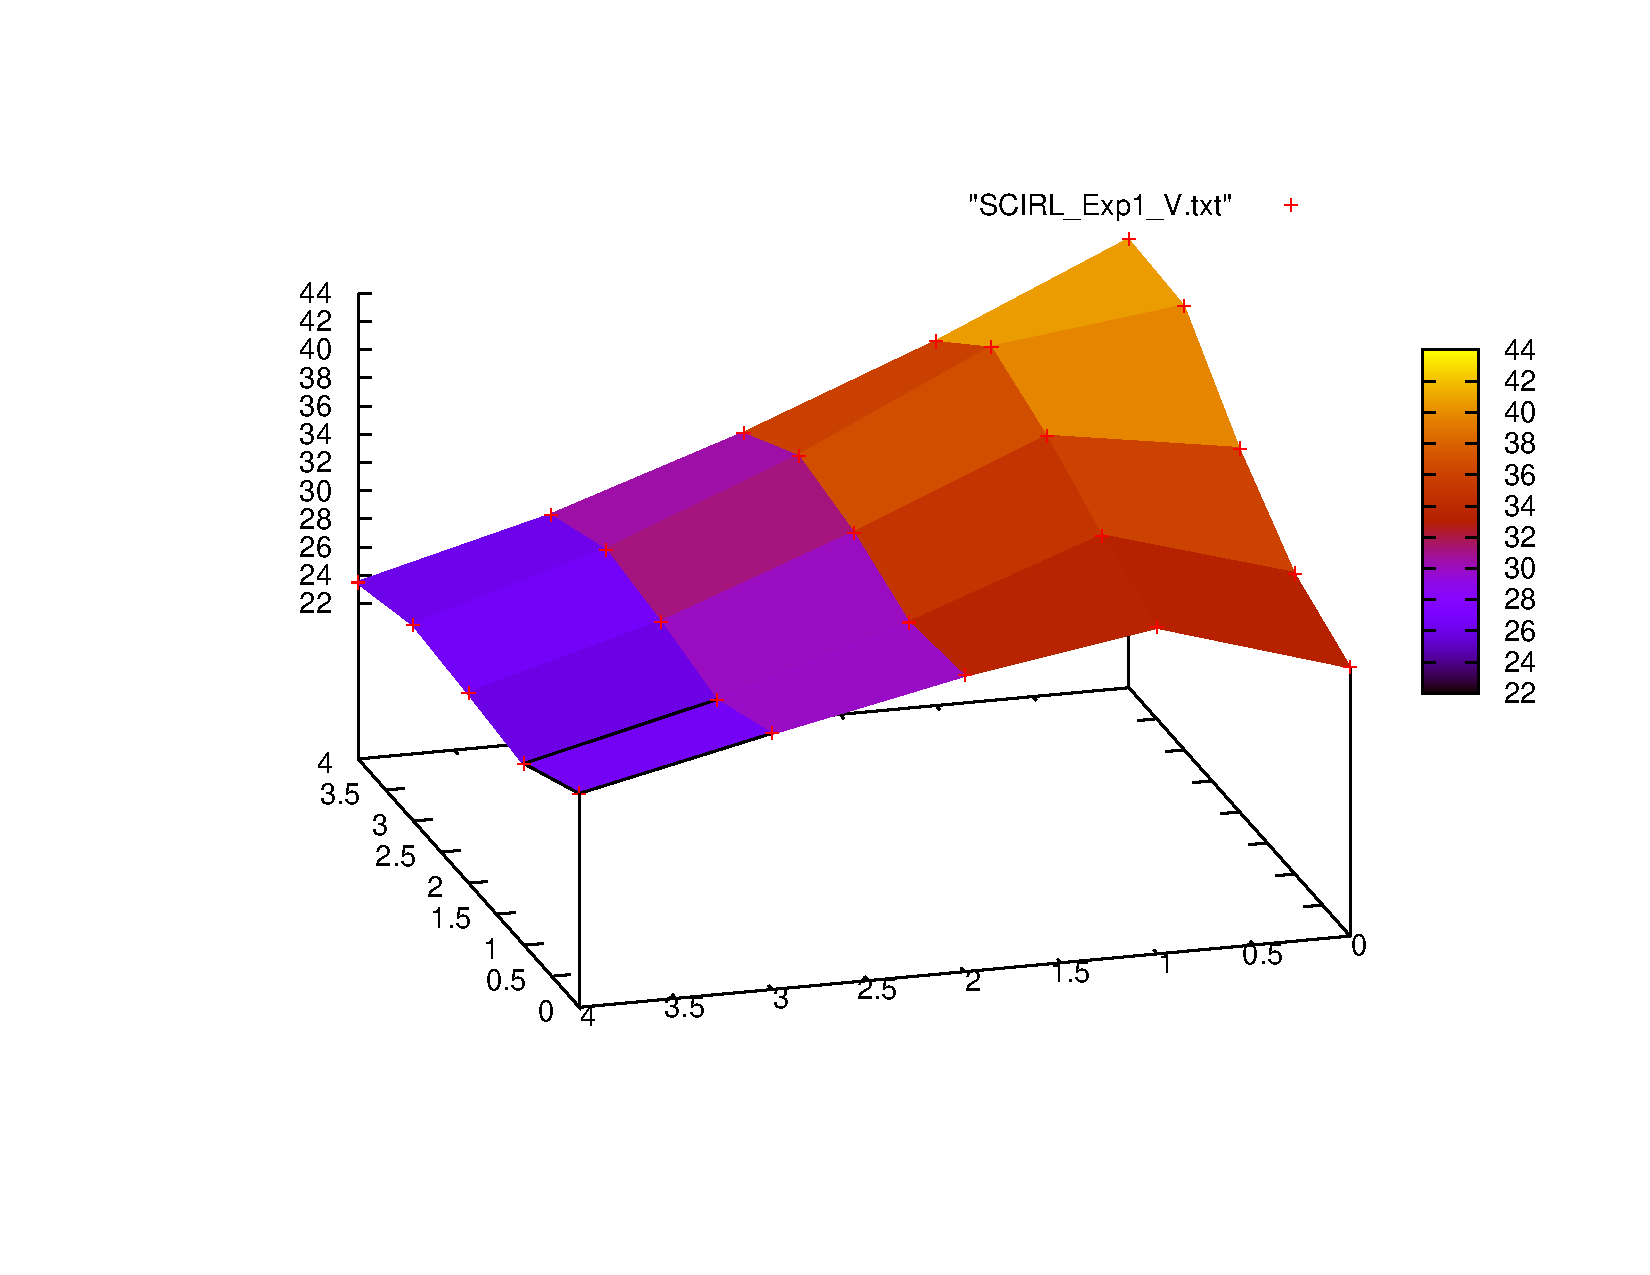
\includegraphics[width=.52\textwidth]{SCIRL_Exp1_V.pdf}
\vspace{-90pt}
%}
      \end{block}
    \end{column}
    \begin{column}{.48\textwidth}
      \begin{block}{11. Inverted Pendulum}
        \centering
        \fontsize{11pt}{11pt}\selectfont
        \resizebox{.95\columnwidth}{!}{

}
\vspace{-70pt}
          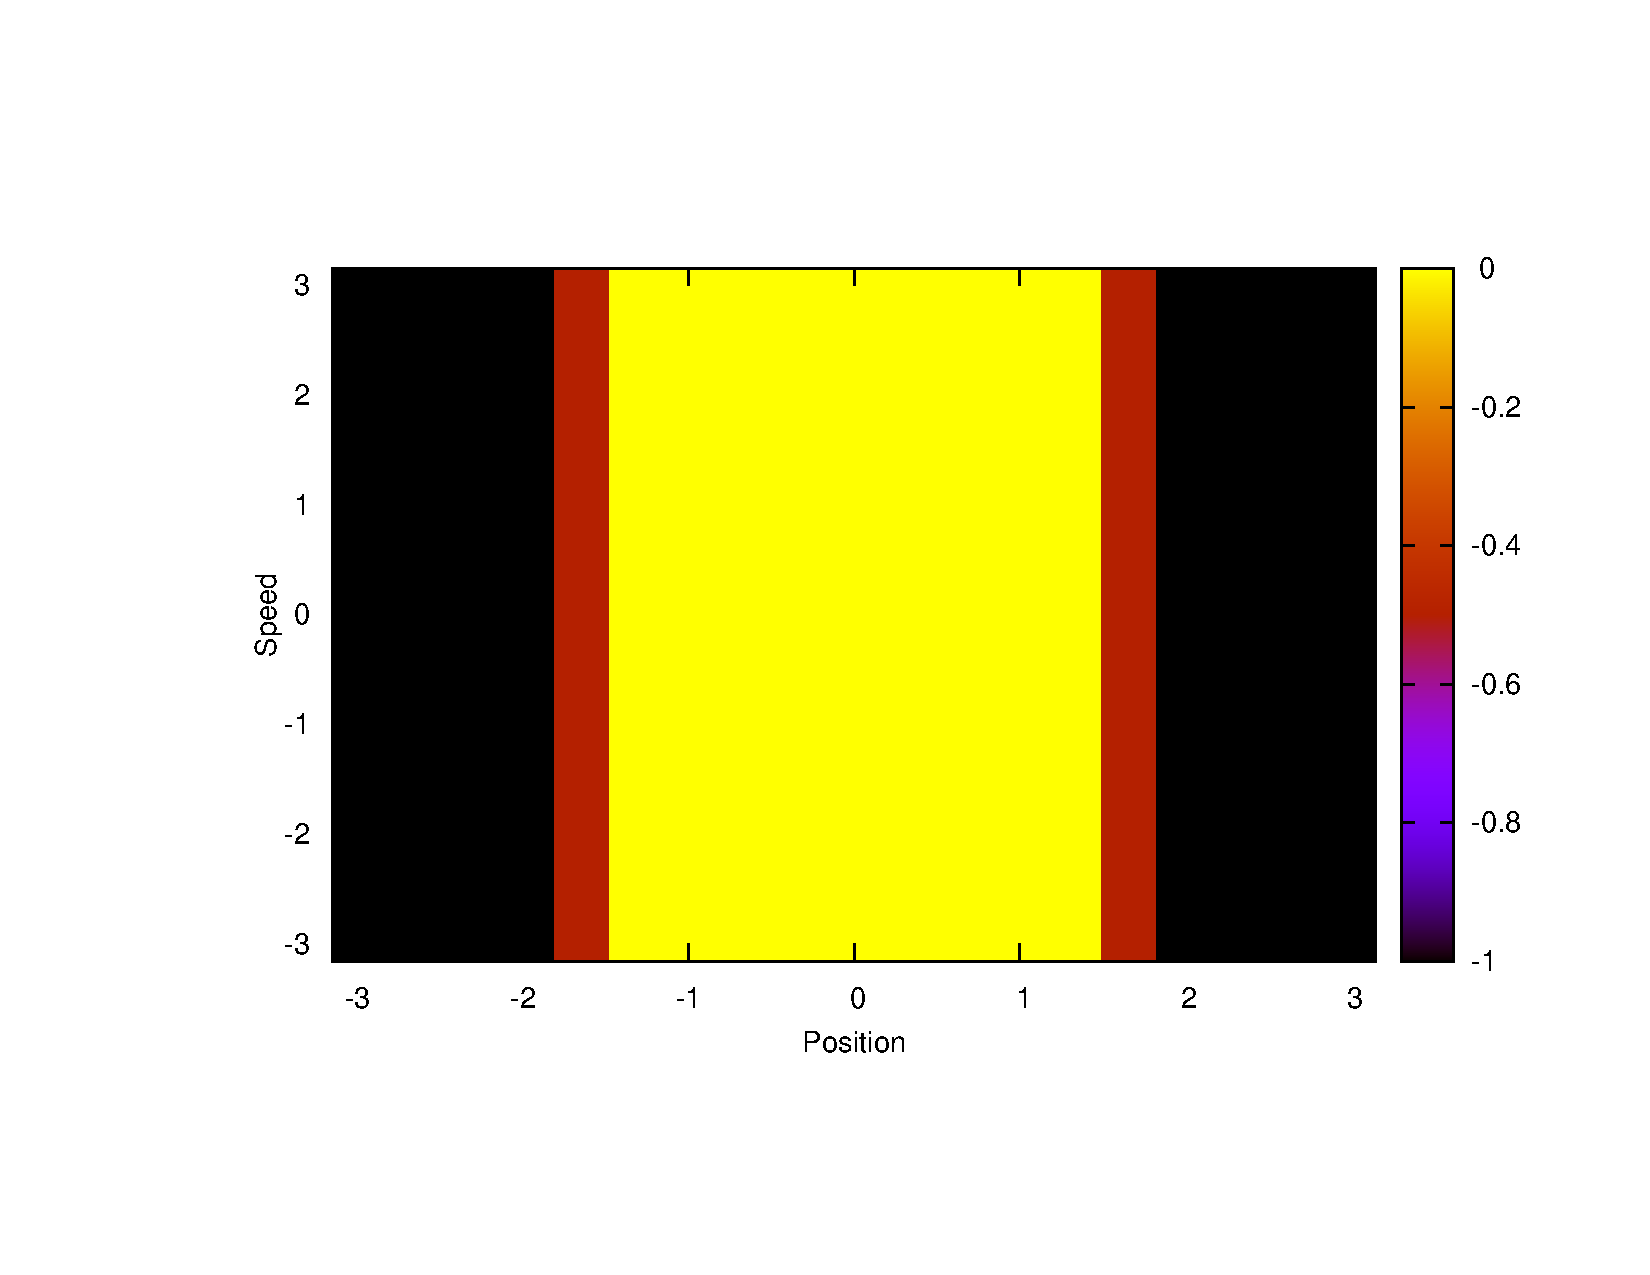
\includegraphics[width=.52\textwidth]{LAFEM_Exp3_true_R}\hspace{-100pt}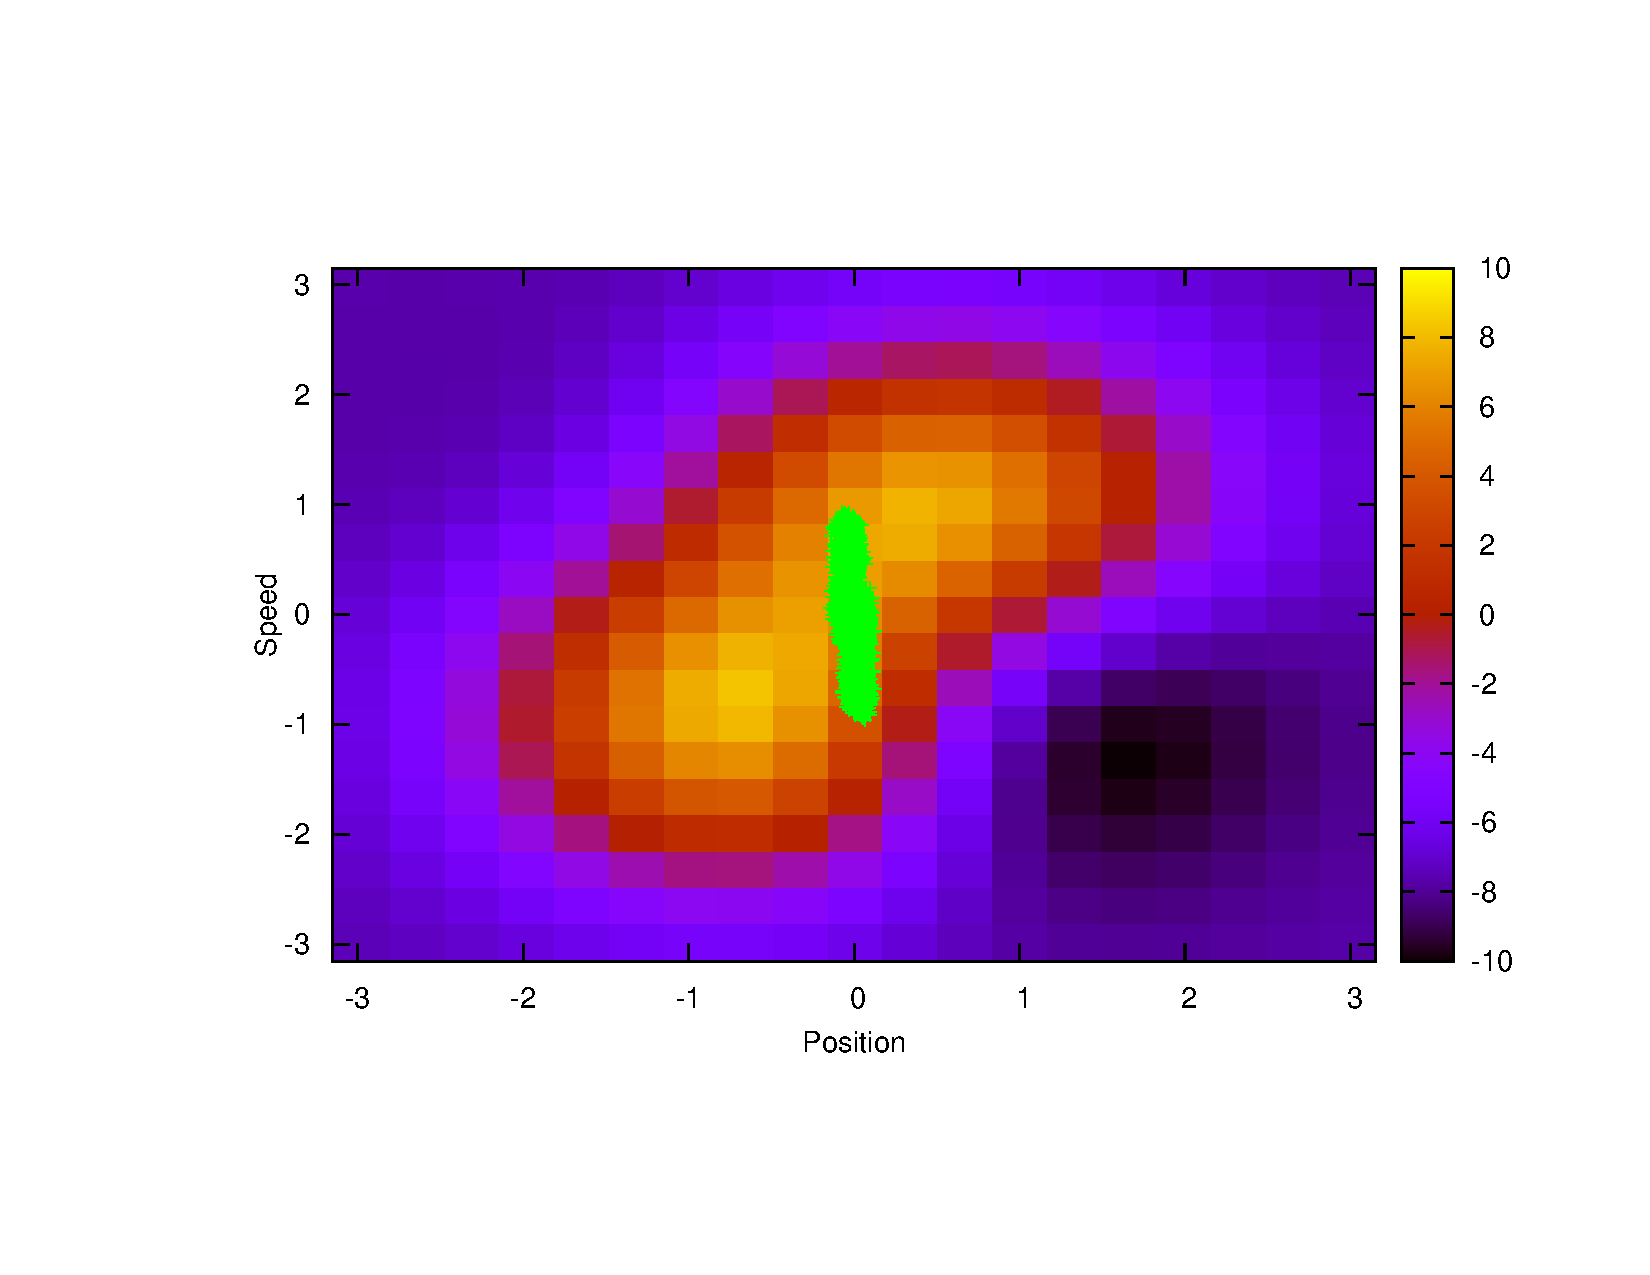
\includegraphics[width=.52\textwidth]{LAFEM_Exp3_lafem_R}\\
%          Blah
\vspace{-110pt}
          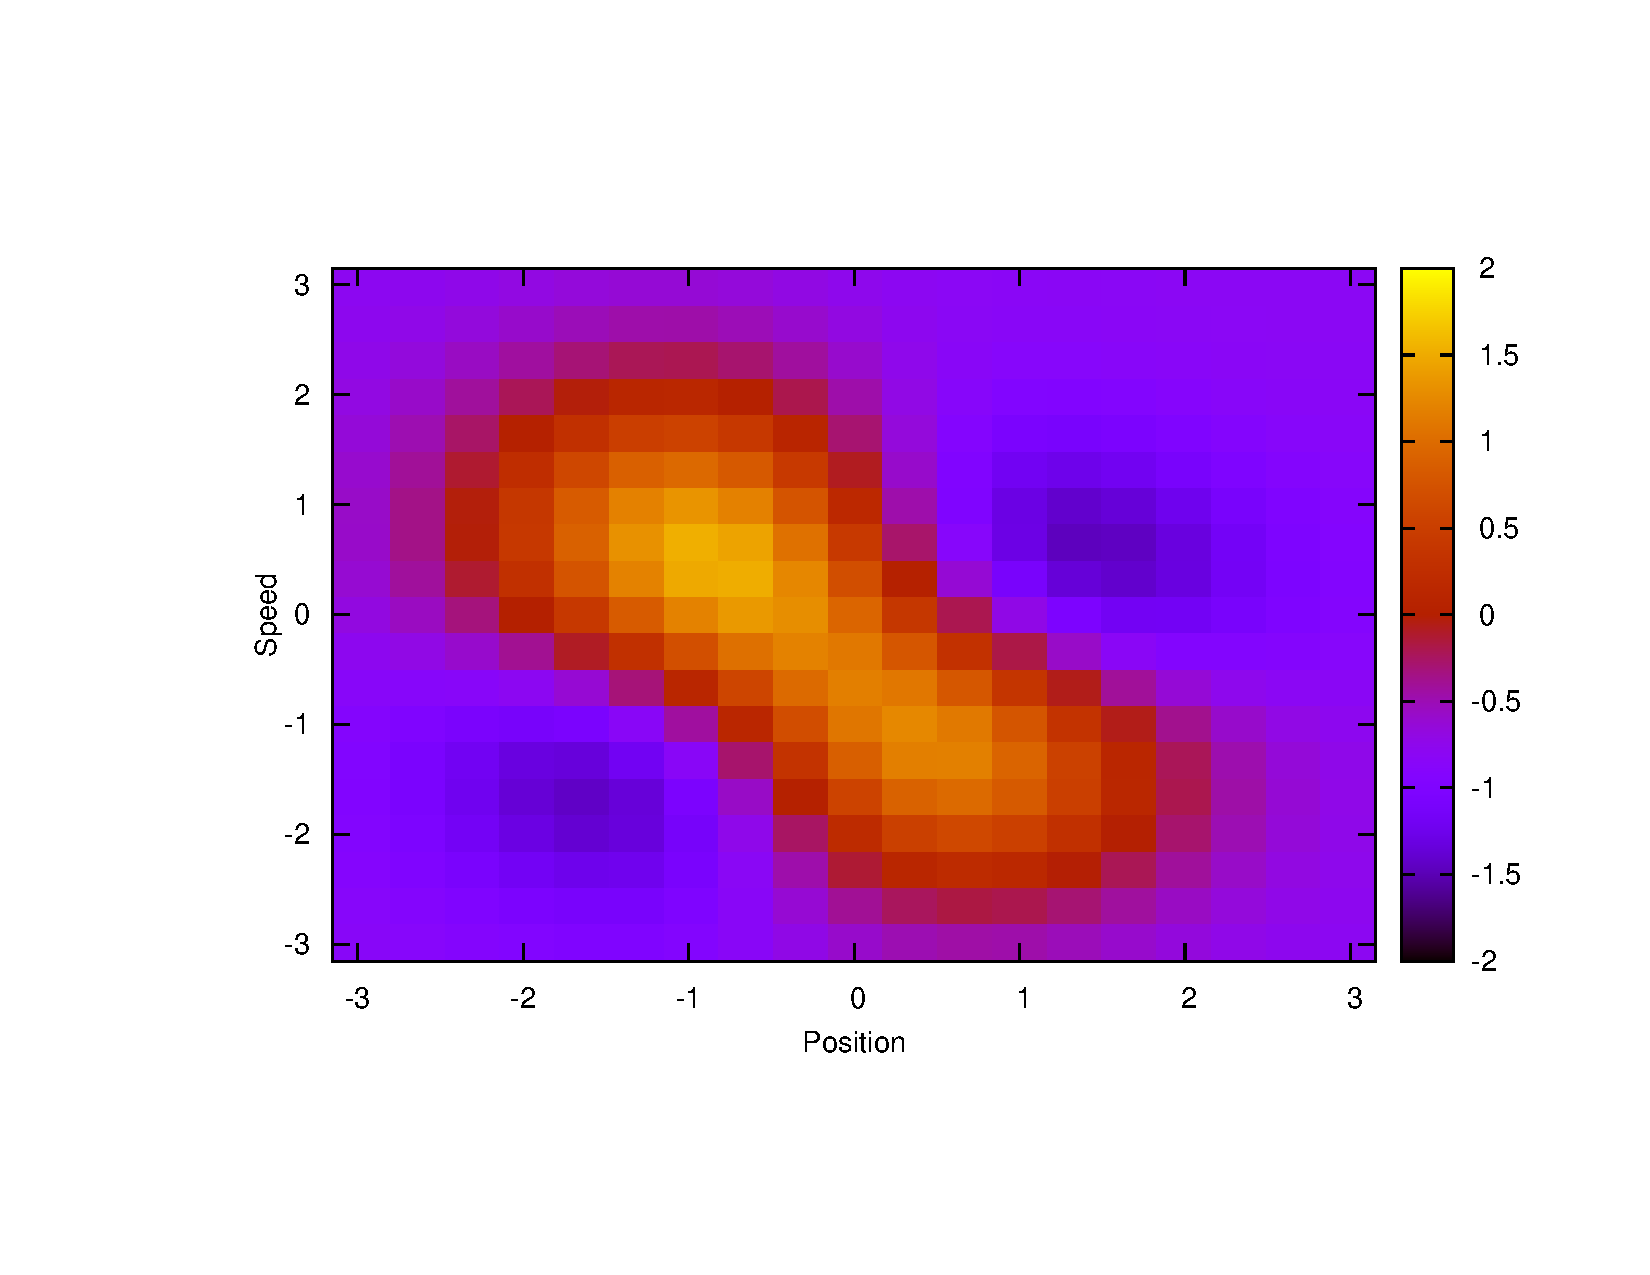
\includegraphics[width=.52\textwidth]{LAFEM_Exp3_Vexpert}\hspace{-100pt}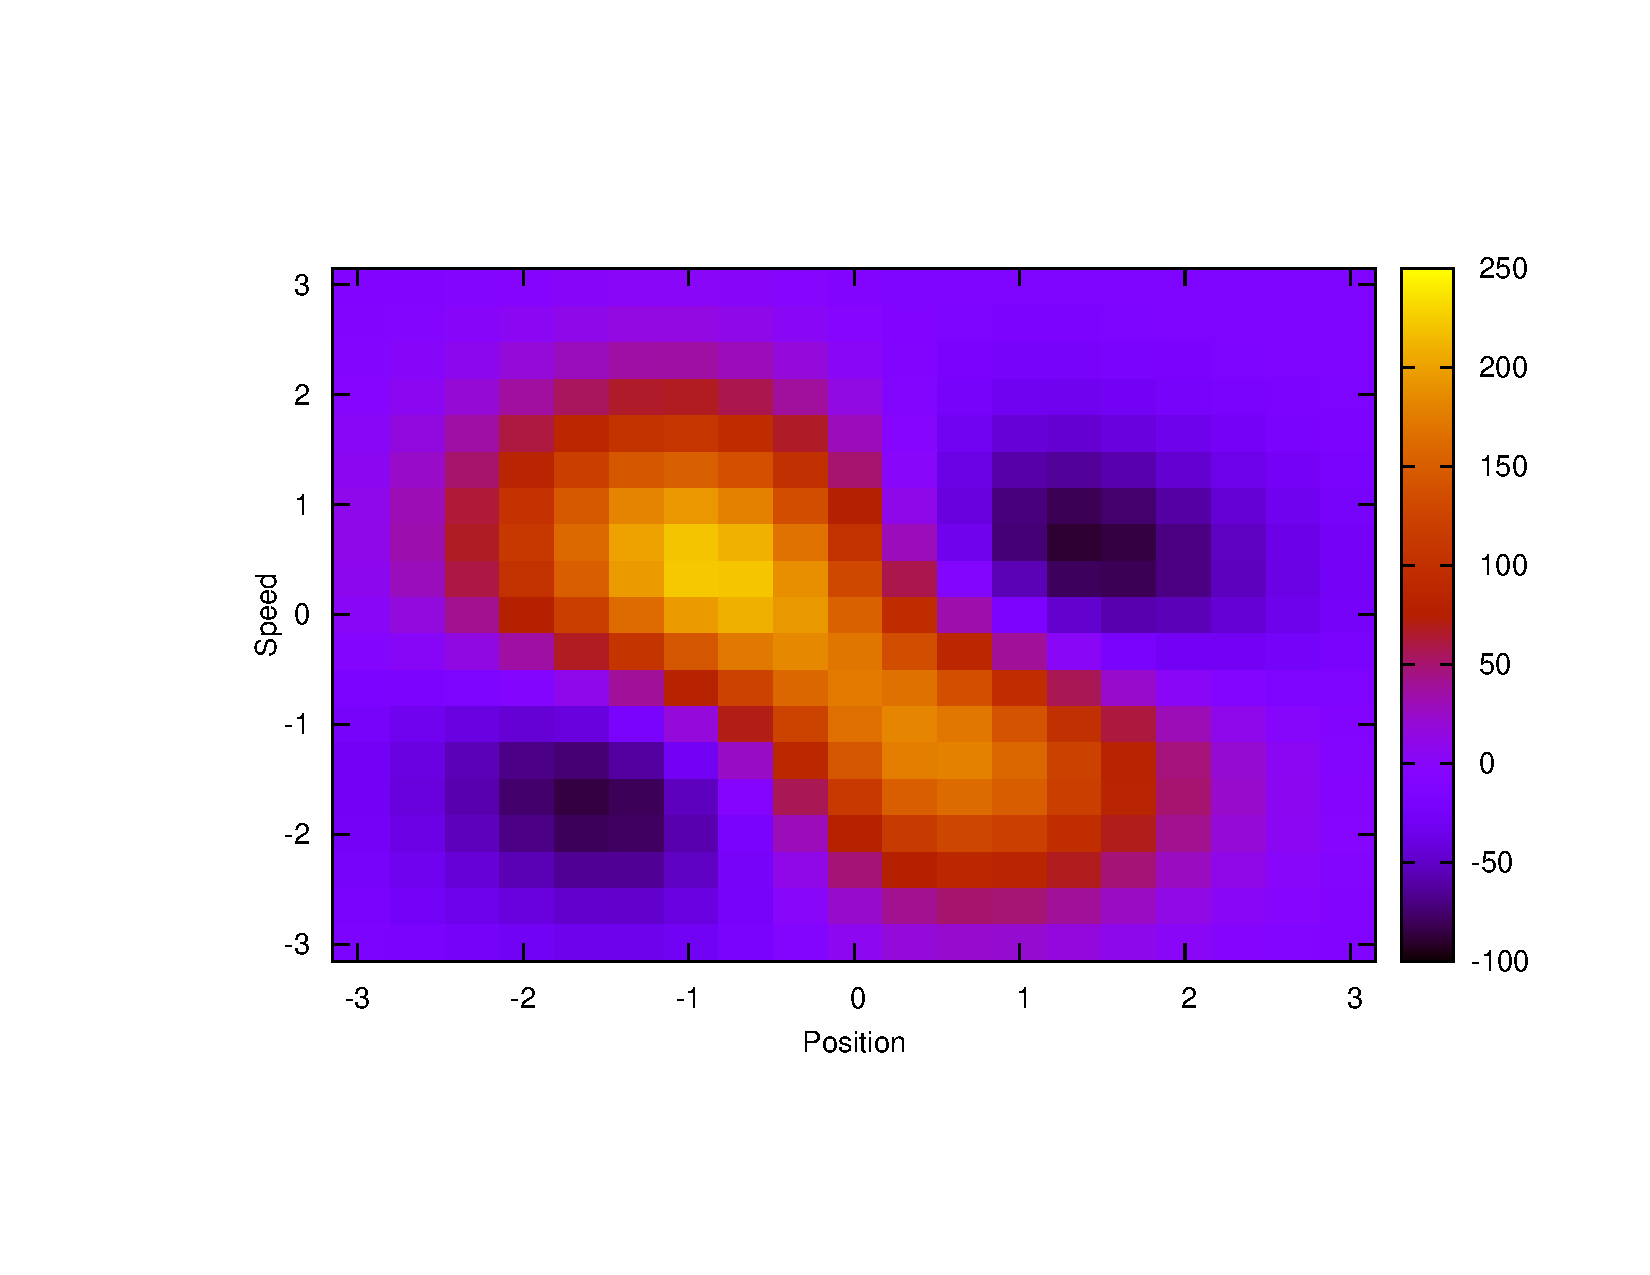
\includegraphics[width=.52\textwidth]{LAFEM_Exp3_Vagent}
\vspace{-90pt}
%}
      \end{block}
    \end{column}
  \end{columns}



\end{frame}
\end{document}
